Structural colors in nature and man-made photonic crystals have provided beautiful examples of the interaction between light and matter.
In the cases of periodic structures, especially those composed of spheres, relatively straight forward calculations are sufficient to predict which colors of light will constructively interfere upon scattering.
With the realization that non-periodic structures can also cause selective scattering and the development of synthesis techniques for producing large numbers of optical-scale non-spherical particles, I have tried to broaden our concept of structural colors and photonic crystals.

\section{Isotropic Structural Color}
Non-iridescent structural color is realized when an isotropic structure has a peak in $I(q)$ and wavelength-independent scattering is suppressed.
We use a bidisperse mixture of spheres to frustrate crystallization and produce an isotropic structure.
We find that controlling film thickness or absorption length are effective at enhancing contrast in reflectance spectra.
These films may have applications in coatings, cosmetics and textiles.
While the basic optical properties of structurally-colored feathers have been reproduced, more work must be done before the biomimetic samples perform as well as their biological counterparts.

I believe that the most significant cause of the difference in performance between our biomimetic structures and those found in feathers is the inverse arrangement of high and low indices of refraction.
Specifically, the scattering at short wavelengths produced by the colloid films is enhanced by the fact that the spheres have a higher index of refraction than their surroundings.
The local index of refraction environment has been shown to have a significant impact on the scattering behavior of these types of materials \cite{Liew:2011}.
The most obvious way to test this would be to invert the biomimetic structures to create an array of low index spheres in a high index background.
There are methods that have been used to create inverse opals which involve the infiltration of an inorganic liquid precursor into a pre-formed colloidal crystal which undergoes a sol-gel reaction to fill the voids between particles with a material such as titania or silica \cite{Schroden:2002}.
The infiltration and deposition step is followed by heating the composite material to a temperature high enough to cause depolymerization and evaporation of the polymer template, leaving behind an inverted structure.
Both of these steps generate significant stresses in the original structure and lead to shrinkage and cracking.
Figure~\ref{fig:crackedsilica} shows the results of such a procedure, the small domains left behind after this procedure make it difficult to obtain high quality optical spectra.
A technique that avoids the formation of cracks has been developed \cite{Hatton:2010} and involves depositing the inorganic background material and the colloidal structure simultaneously.
A demonstration of the results of this technique is shown in Figure~\ref{fig:nocracksilica}.
I have been able to produce centimeter-scale areas of crack free silica air-in-silca structures using this procedure.
This technique should allow for the creation of inverted versions of the structures described in Chapter~\ref{chap:sphere-isotropic}, provided that the co-deposition of the background material does not interfere with the formation of the necessary isotropic structures.

\begin{figure*}[htbp]
\centering
%% first subfigure
	\subfloat[SEM image of a colloidal crystal before infiltration.]{
		\label{fig:crackedsilica:before}
		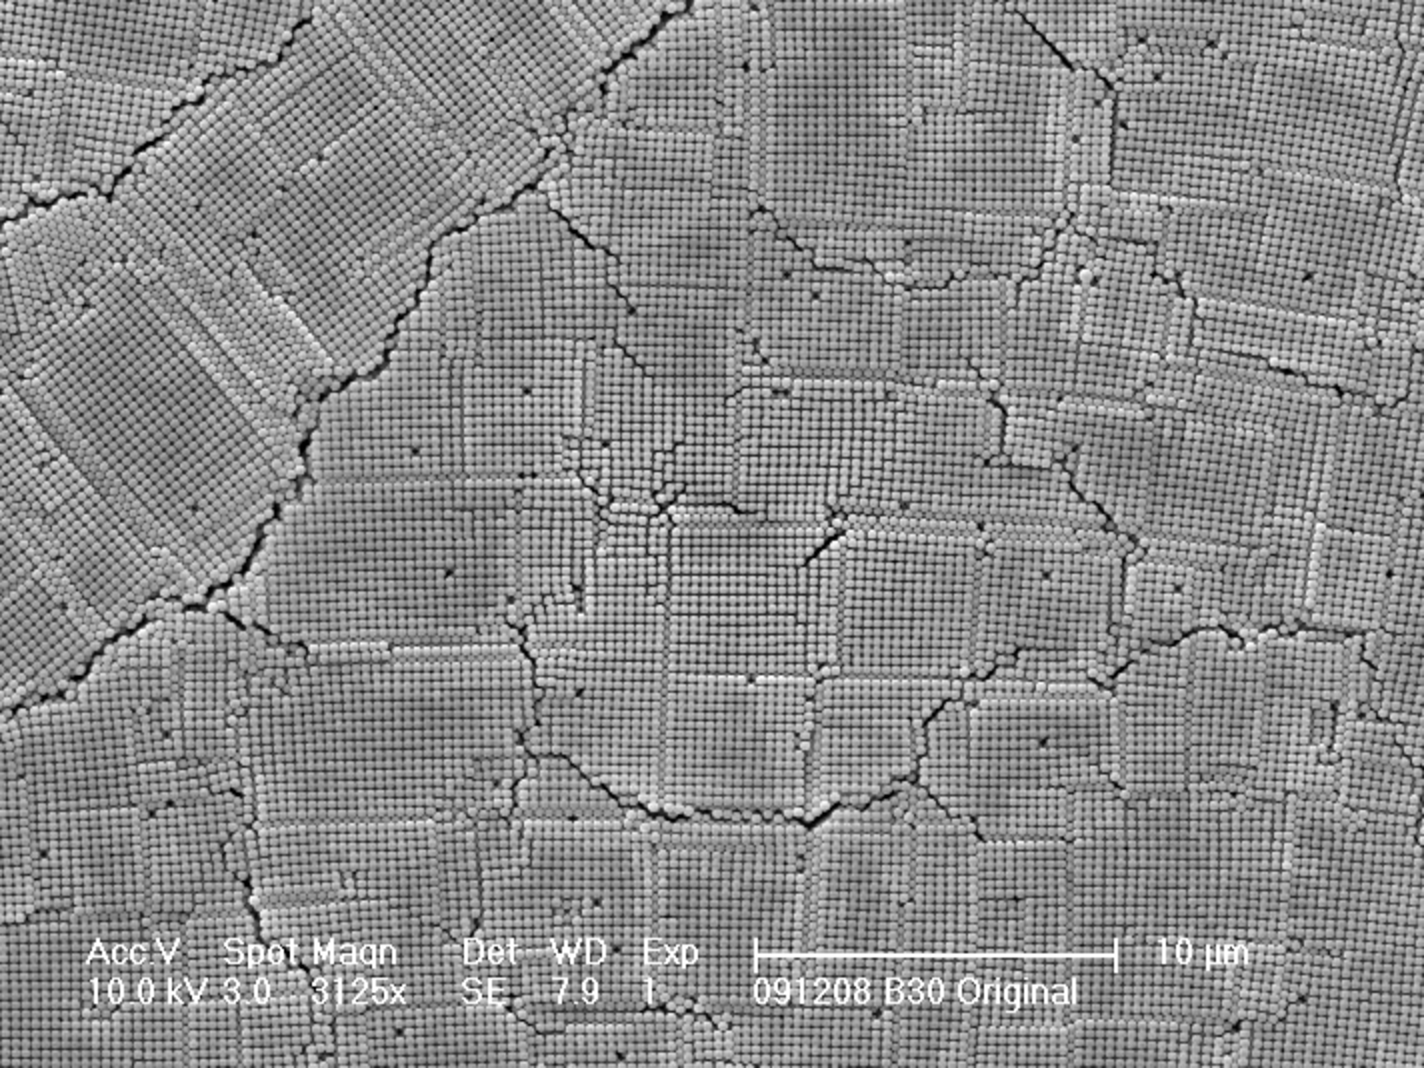
\includegraphics[width=2.75in]{figures/B30Original3125.pdf}}
\hspace{0.25in}	
%% second subfigure
	\subfloat[SEM image of the silica structure after infiltration and burn-out following a procedure similar to that described in Ref.~\cite{Schroden:2002}.]{
		\label{fig:crackedsilica:after}
		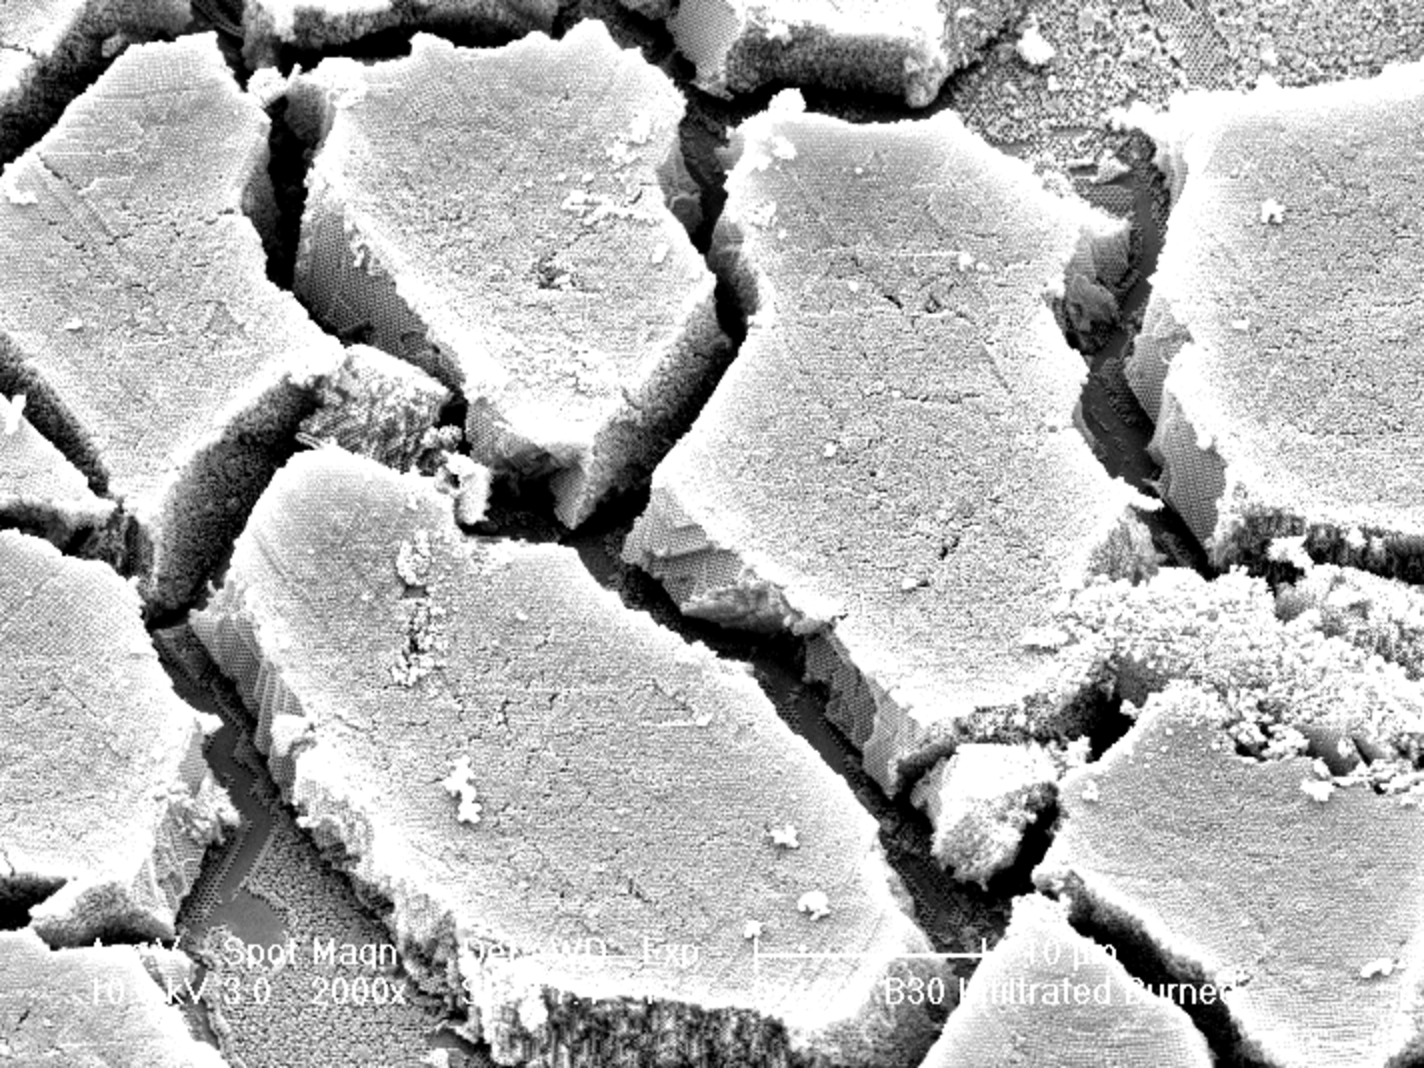
\includegraphics[width=2.75in]{figures/B30InverseCrack2000.pdf}}
\caption{\label{fig:crackedsilica}\emph{Traditional inversion techniques cause cracking.}}
\end{figure*} 

\begin{figure*}[htbp]
\centering
	\subfloat[SEM image of colloidal crystal prepared following the methods in Ref.~\cite{Hatton:2010}.]{
	\label{fig:nocracksilica:before}
	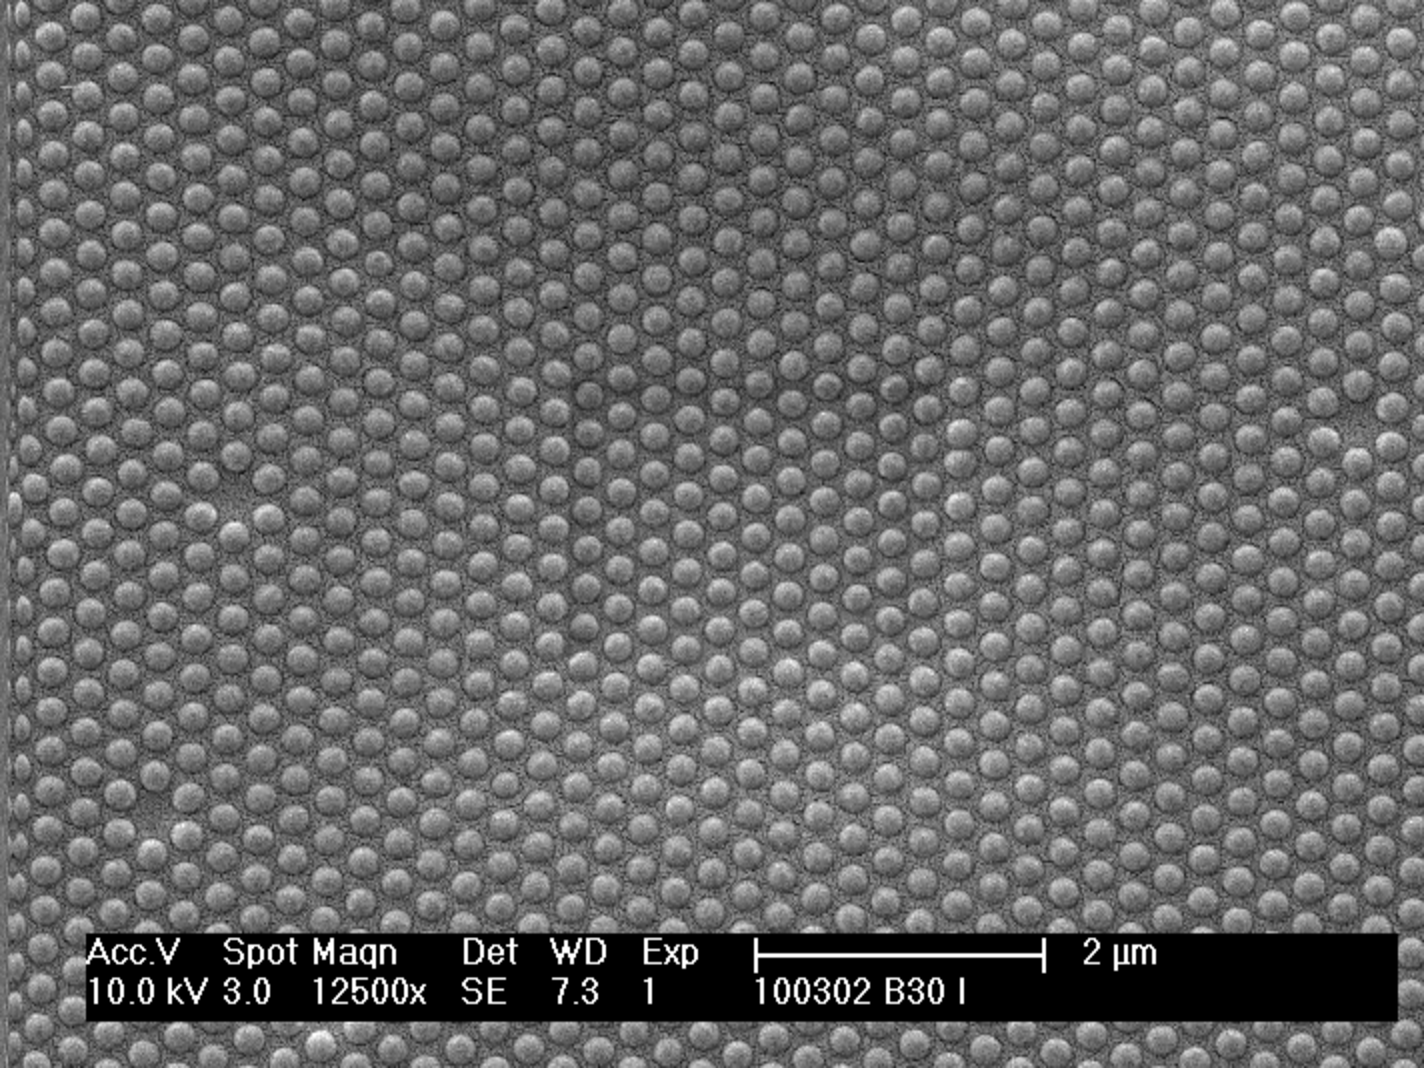
\includegraphics[width=2.75in]{figures/B30FilledNew12500.pdf}}
\hspace{0.25in}
	\subfloat[SEM image of the inverse structure achieved after burn-out following Ref.~\cite{Hatton:2010}.]{
	\label{fig:nocracksilica:after}
	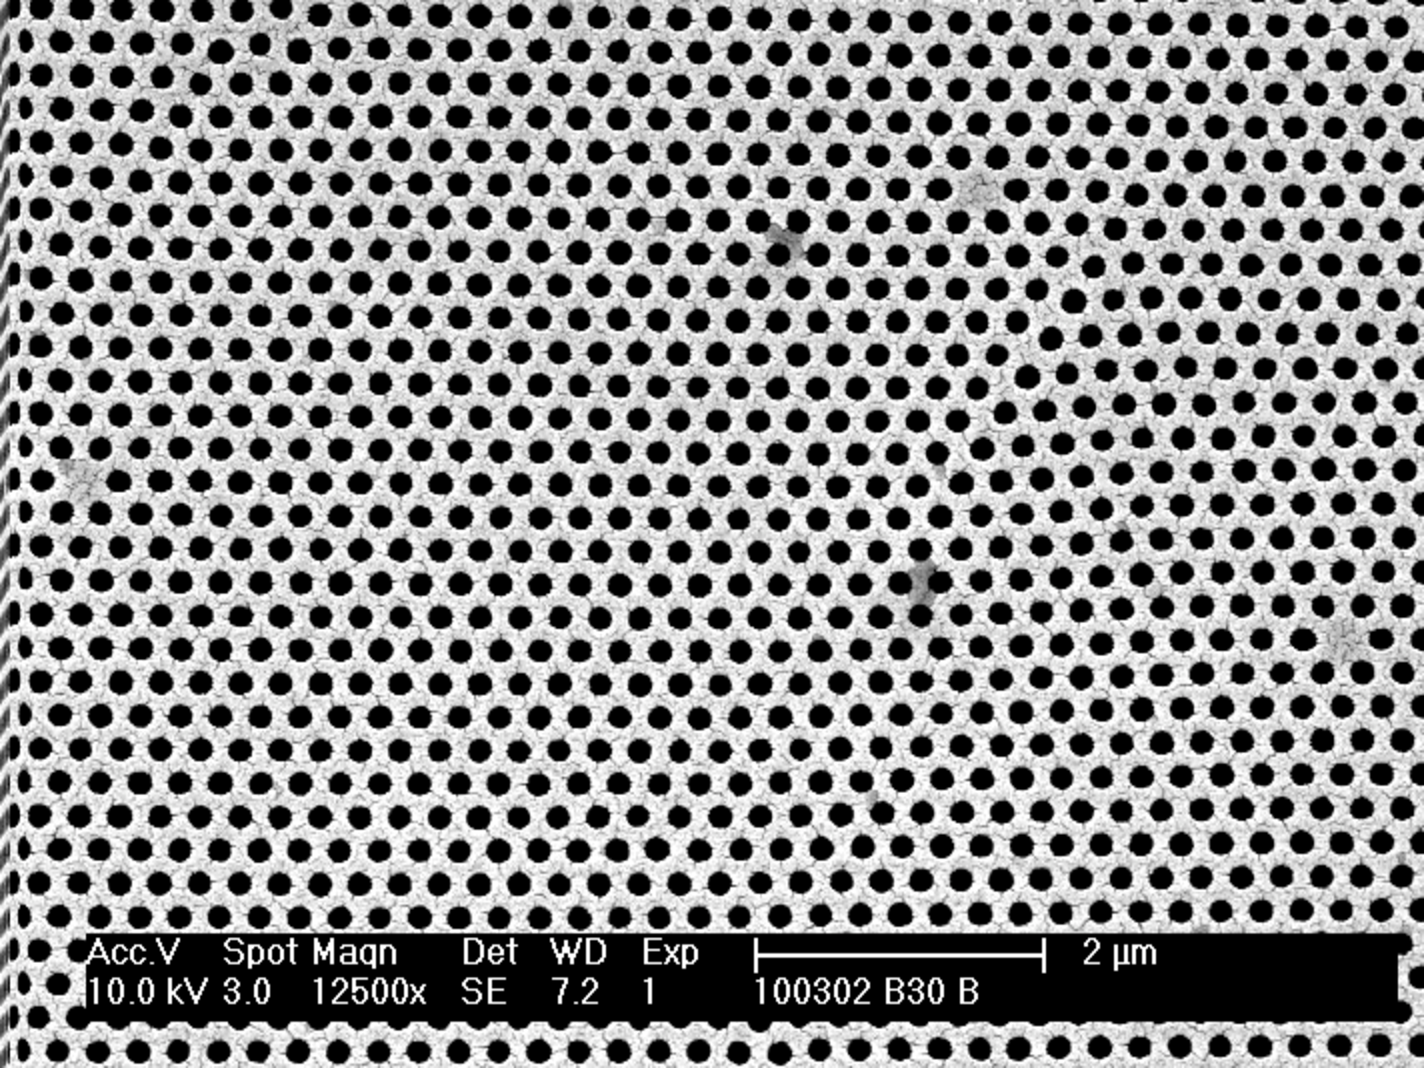
\includegraphics[width=2.75in]{figures/B30InverseNew12500.pdf}}\\[0.25in]
	\subfloat[Low-magnification SEM image of inverse structure.]{
	\label{fig:nocracksilica:after:low}
	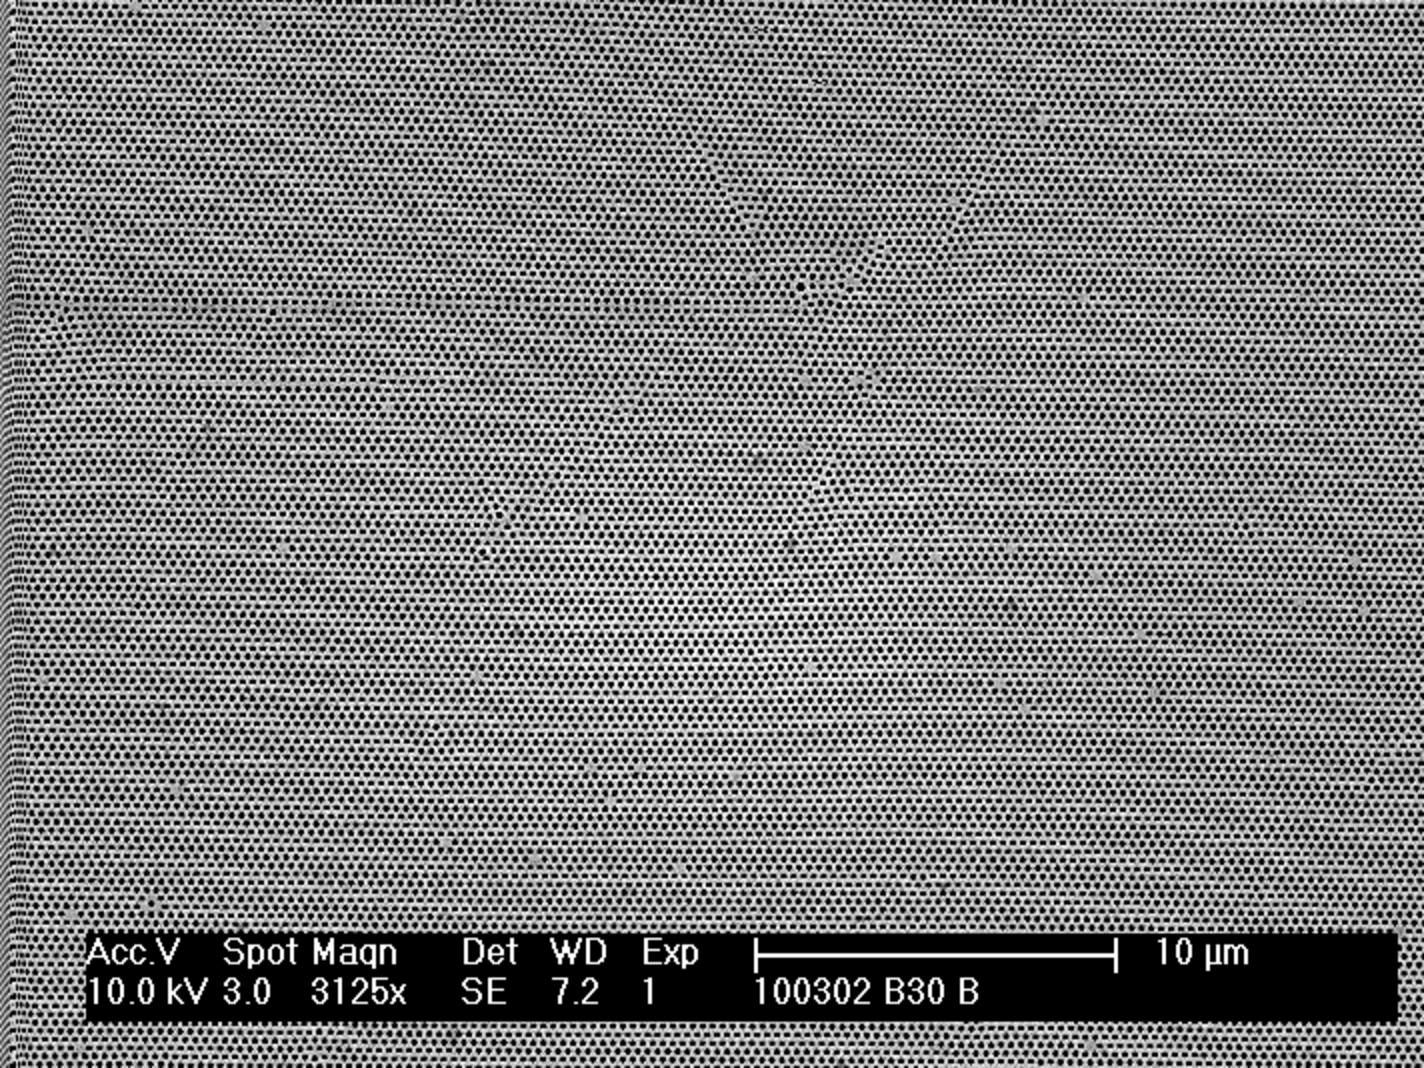
\includegraphics[width=4in]{figures/B30InverseNew3125.pdf}}
\caption{\label{fig:nocracksilica}\emph{Simultaneous deposition of inorganic background and colloidal template prevents cracking.}}
\end{figure*}

Another exciting possibility for an application of isotropic structural colors may result from the combination of this work with other research from our lab on the electrostatic interactions of colloids in non-polar solvents \cite{Sainis:2008, Sainis:2008:2, Merrill:2009}.
One conclusion drawn from studying the electrostatics of particles in non-polar solvents is that the interaction between a pair of particles is influenced by the presence of a third particle in a way that is not pair-wise additive \cite{Merrill:2009}.
We expect that the presence of an external field will also influence the interaction of particles in oil.
The idea, then, is that the spacing between particles in a dense suspension can be tuned by applying an external electric field.
With particle sizes and separations the right scale to scatter visible light, it may be possible to build a device displaying isotropic structural color that can be altered dynamically by varying an applied electric field.


\section{Dumbbell Crystals}
We describe the self assembly of non-spherical particles into crystals with novel structure and optical properties combining a partial photonic bandgap with birefringence that can be  modulated by an external field or quenched by solvent evaporation. 
Specifically, we study symmetric optical scale polymer dumbbells with an aspect ratio of 1.58. 
Hard particles with this geometry have been predicted to crystallize in equilibrium at high concentrations.
However, experiments have shown that unlike spherical particles which readily crystallize in the bulk, these dumbbells crystallize only under strong confinement - in thin films less than three particles thick.
Here, we demonstrate the use of an external electric field to align and assemble the dumbbells to make a birefringent suspension with structural color.
When the electric field is turned off, the dumbbells rapidly lose their orientational order and the color and birefringence quickly go away.
In this way, dumbbells combine the structural color of photonic crystals with the field addressability of liquid crystals.
In addition, we find that if the solvent is removed in the presence of an electric field, the particles self assemble into a novel, dense crystalline packing hundreds of particles thick.
Analysis of the crystal structure indicates that the dumbbells have a packing fraction of 0.7862, higher than the densest known packings of spheres and ellipsoids.
We perform numerical experiments that demonstrate the importance of controlling the orientation of the dumbbells during drying for crystal formation.

The response of a suspension of dumbbells to an AC electric field described in Chapter~\ref{chap:dumbbell-crystal} is quite striking.
However, before this system can be developed into a useful optical device, it is necessary to have a clearer idea of the structures formed in suspension.
Based on the optical properties of the suspension in a field, it seems reasonable that the structure is crystalline, but without a direct measurement we cannot be certain about the exact structure.
The SAXS technique we use to study the structurally-colored materials in Chapter~\ref{chap:sphere-isotropic} could be used to study the structures formed by dumbbells in external fields.
It would be interesting to explore the possibility of annealing the crystal structure formed in an electric field by cycling the field on and off..
Finally, optimizing the speed with which the birefringence and structural color can be switched on and off by working with higher volume fractions, smaller chamber dimensions, or stronger fields would help in identifying potential applications for such a device.


\section{Beyond Photonics}

The size and shape of the dumbbells used in this dissertation have allowed us to assemble a new type of photonic crystal.
The synthesis procedure described in Ref.~\cite{Park2010} and in Appendix~\ref{chap:synthesis} gives us control over the surface chemistry, and hence the hydrophilic/hydrophobic character of each lobe.
For example, the dumbbells used in Chapter~\ref{chap:dumbbell-crystal} inherently possess an anisotropic surface chemistry.
The surface of one of the lobes is the same as the polystyrene-co-trimethoxysilylpropylacrylate (poly(Styrene-co-TMSPA)) core-shell spheres described in \ref{chap:synthesis:cs}.
The TMSPA co-monomer introduces trimethoxysilane groups to the polymer which allows for the covalent attachment of a variety of other chemical species via silane chemistry \cite{DerVoort:1996}.
The second lobe introduced in the final synthesis step is composed of only polystyrene sulfonate and is not susceptible to modification by silylation.
Generally speaking, the difference in surface chemistry between the two lobes at this stage should give them some degree of amphiphilicity, but we can take advantage of the siloxane groups to increase the hydrophobicity of the poly(Styrene-co-TMSPA) lobe.
One species we have done preliminary experiments with is N-[3-(Trimethoxysilyl)propyl]ethylenediamine (AEAPTS).
A detailed analysis of the properties of these ``amphiphilic" dumbbells has yet to be carried out so I will refrain from an in-depth description of them.
I will, however, describe a few examples of the behavior of these dumbbells at an oil/water interface.

\begin{figure*}[htbp]
\centering
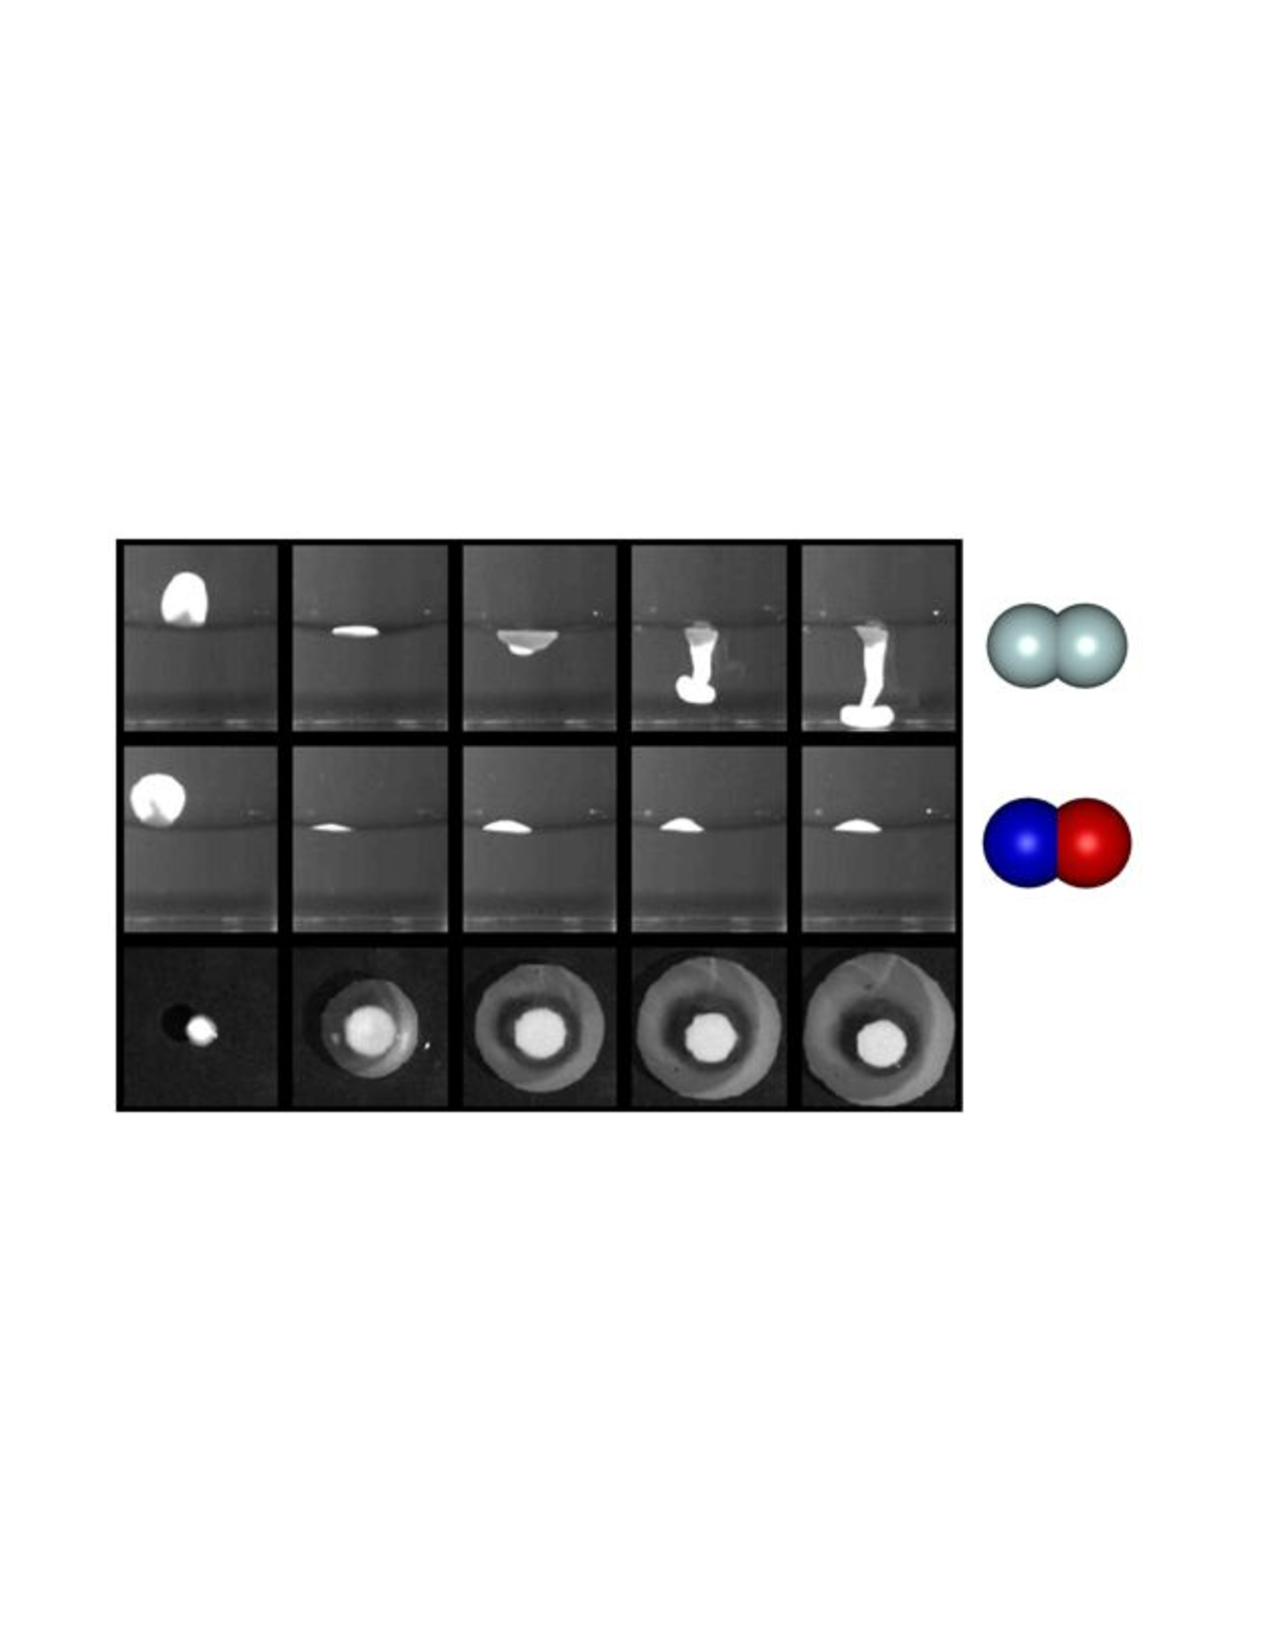
\includegraphics[width=1\textwidth]{figures/dumbbellinterface1.pdf}
\caption{\label{fig:NDBinterface1} \emph{Amphiphilic dumbbells spread at an oil/water interface}
\emph{Top Row:} Still frames from a side-view movie of an aqueous droplet of dumbbells with an isotropic surface chemistry impacting an oil/water interface.
\emph{Middle Row:} Still frames from a side-view movie of an aqueous droplet of dumbbells with an amphiphilic surface chemistry impacting an oil/water interface.
\emph{Bottom Row:} Still frames from a top-view movie of an aqueous droplet of dumbbells with an amphiphilic surface chemistry impacting an oil/water interface.
Frames in each row are separated from each other by 42 ms. The first image in the bottom row is 11 s after the drop impacted the interface.}
\end{figure*}

One demonstration of the affinity of amphiphilic dumbbells for oil/water interfaces is presented in Figure~\ref{fig:NDBinterface1}.
When an aqueous droplet containing dumbbells with an isotropic surface chemistry (produced by introducing a mixture of styrene and TMSPA monomers in the final swelling step, see Appendix~\ref{chap:synthesis:db})impacts the interface between oil (hexadecane) and water, the particles enter the water phase as a droplet and eventually spread by diffusion and convection.
A droplet containing the amphiphilic dumbbells described above behaves very differently.
Upon impact the droplet is trapped at the interface, usually for a few seconds but sometimes as long as five minutes.
At some point the droplet suddenly breaks through the interface but the dumbbells do not enter the water phase.
Instead, they rapidly spread across the oil/water interface and remain at the interface as long as we have observed the sample afterwards, up to about a week.

\begin{figure*}[htbp]
\centering
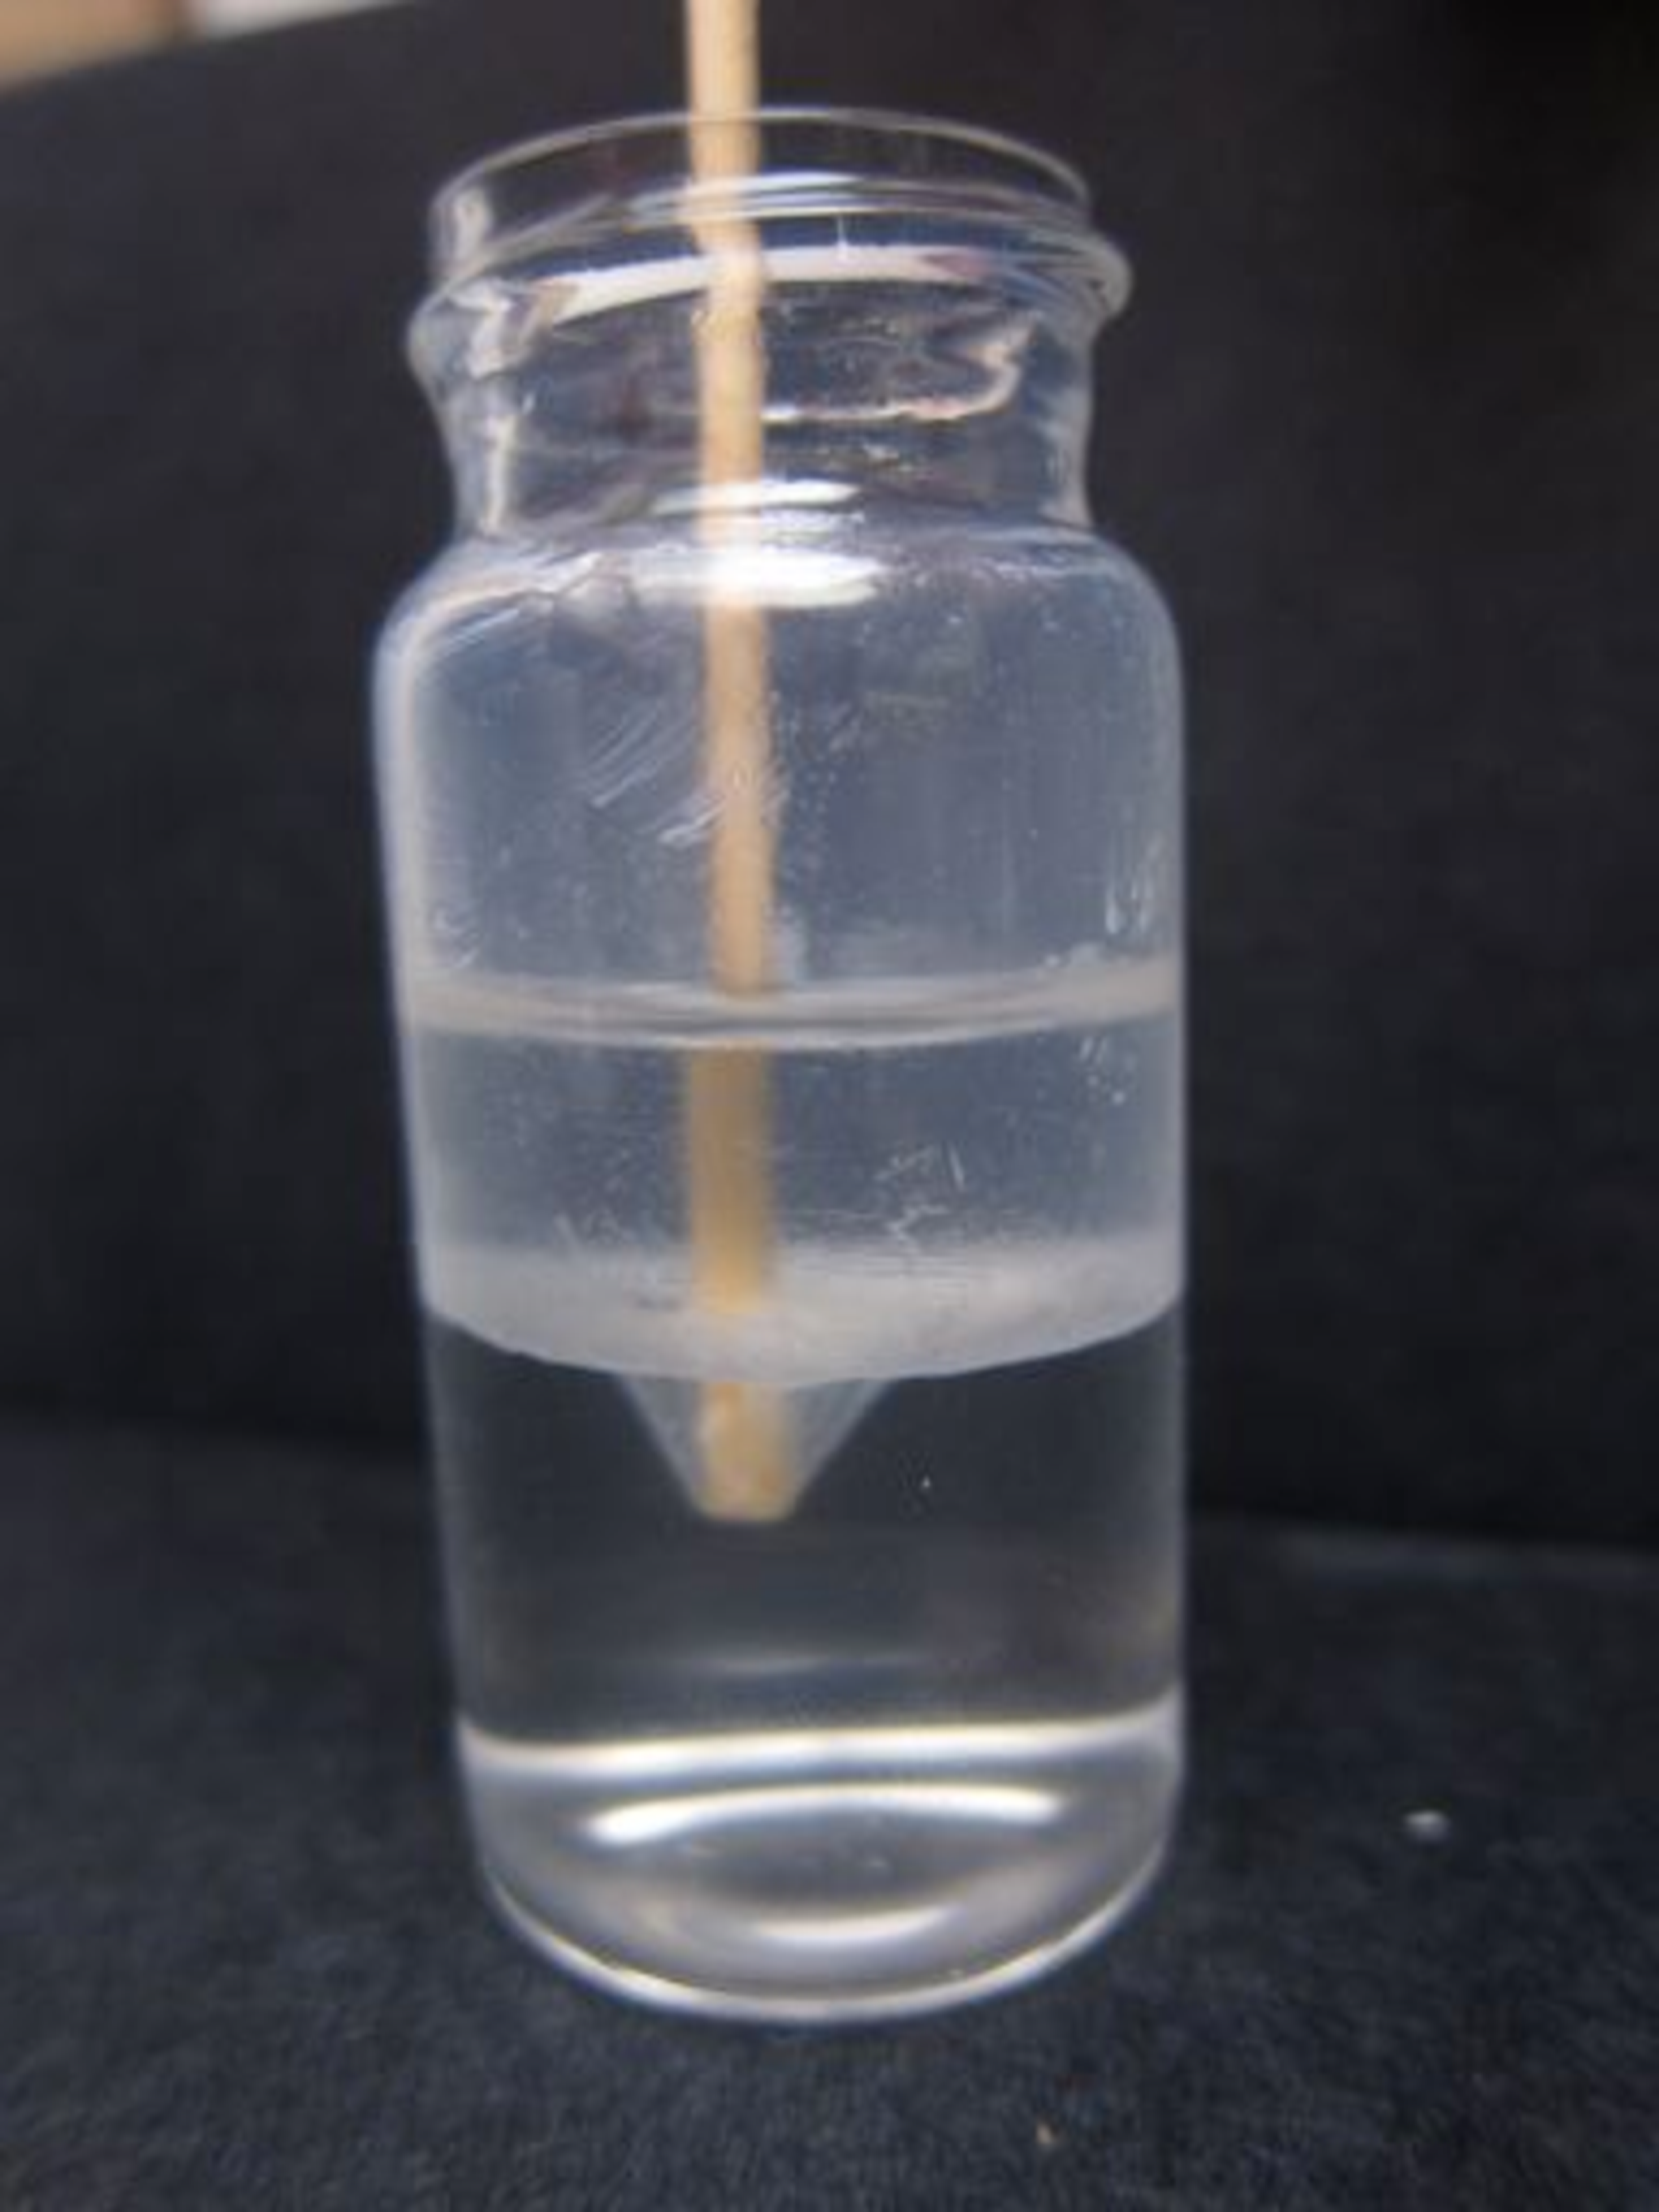
\includegraphics[width=1.25in]{figures/IMG_0911_reduced.pdf}
\hspace{0.2in}
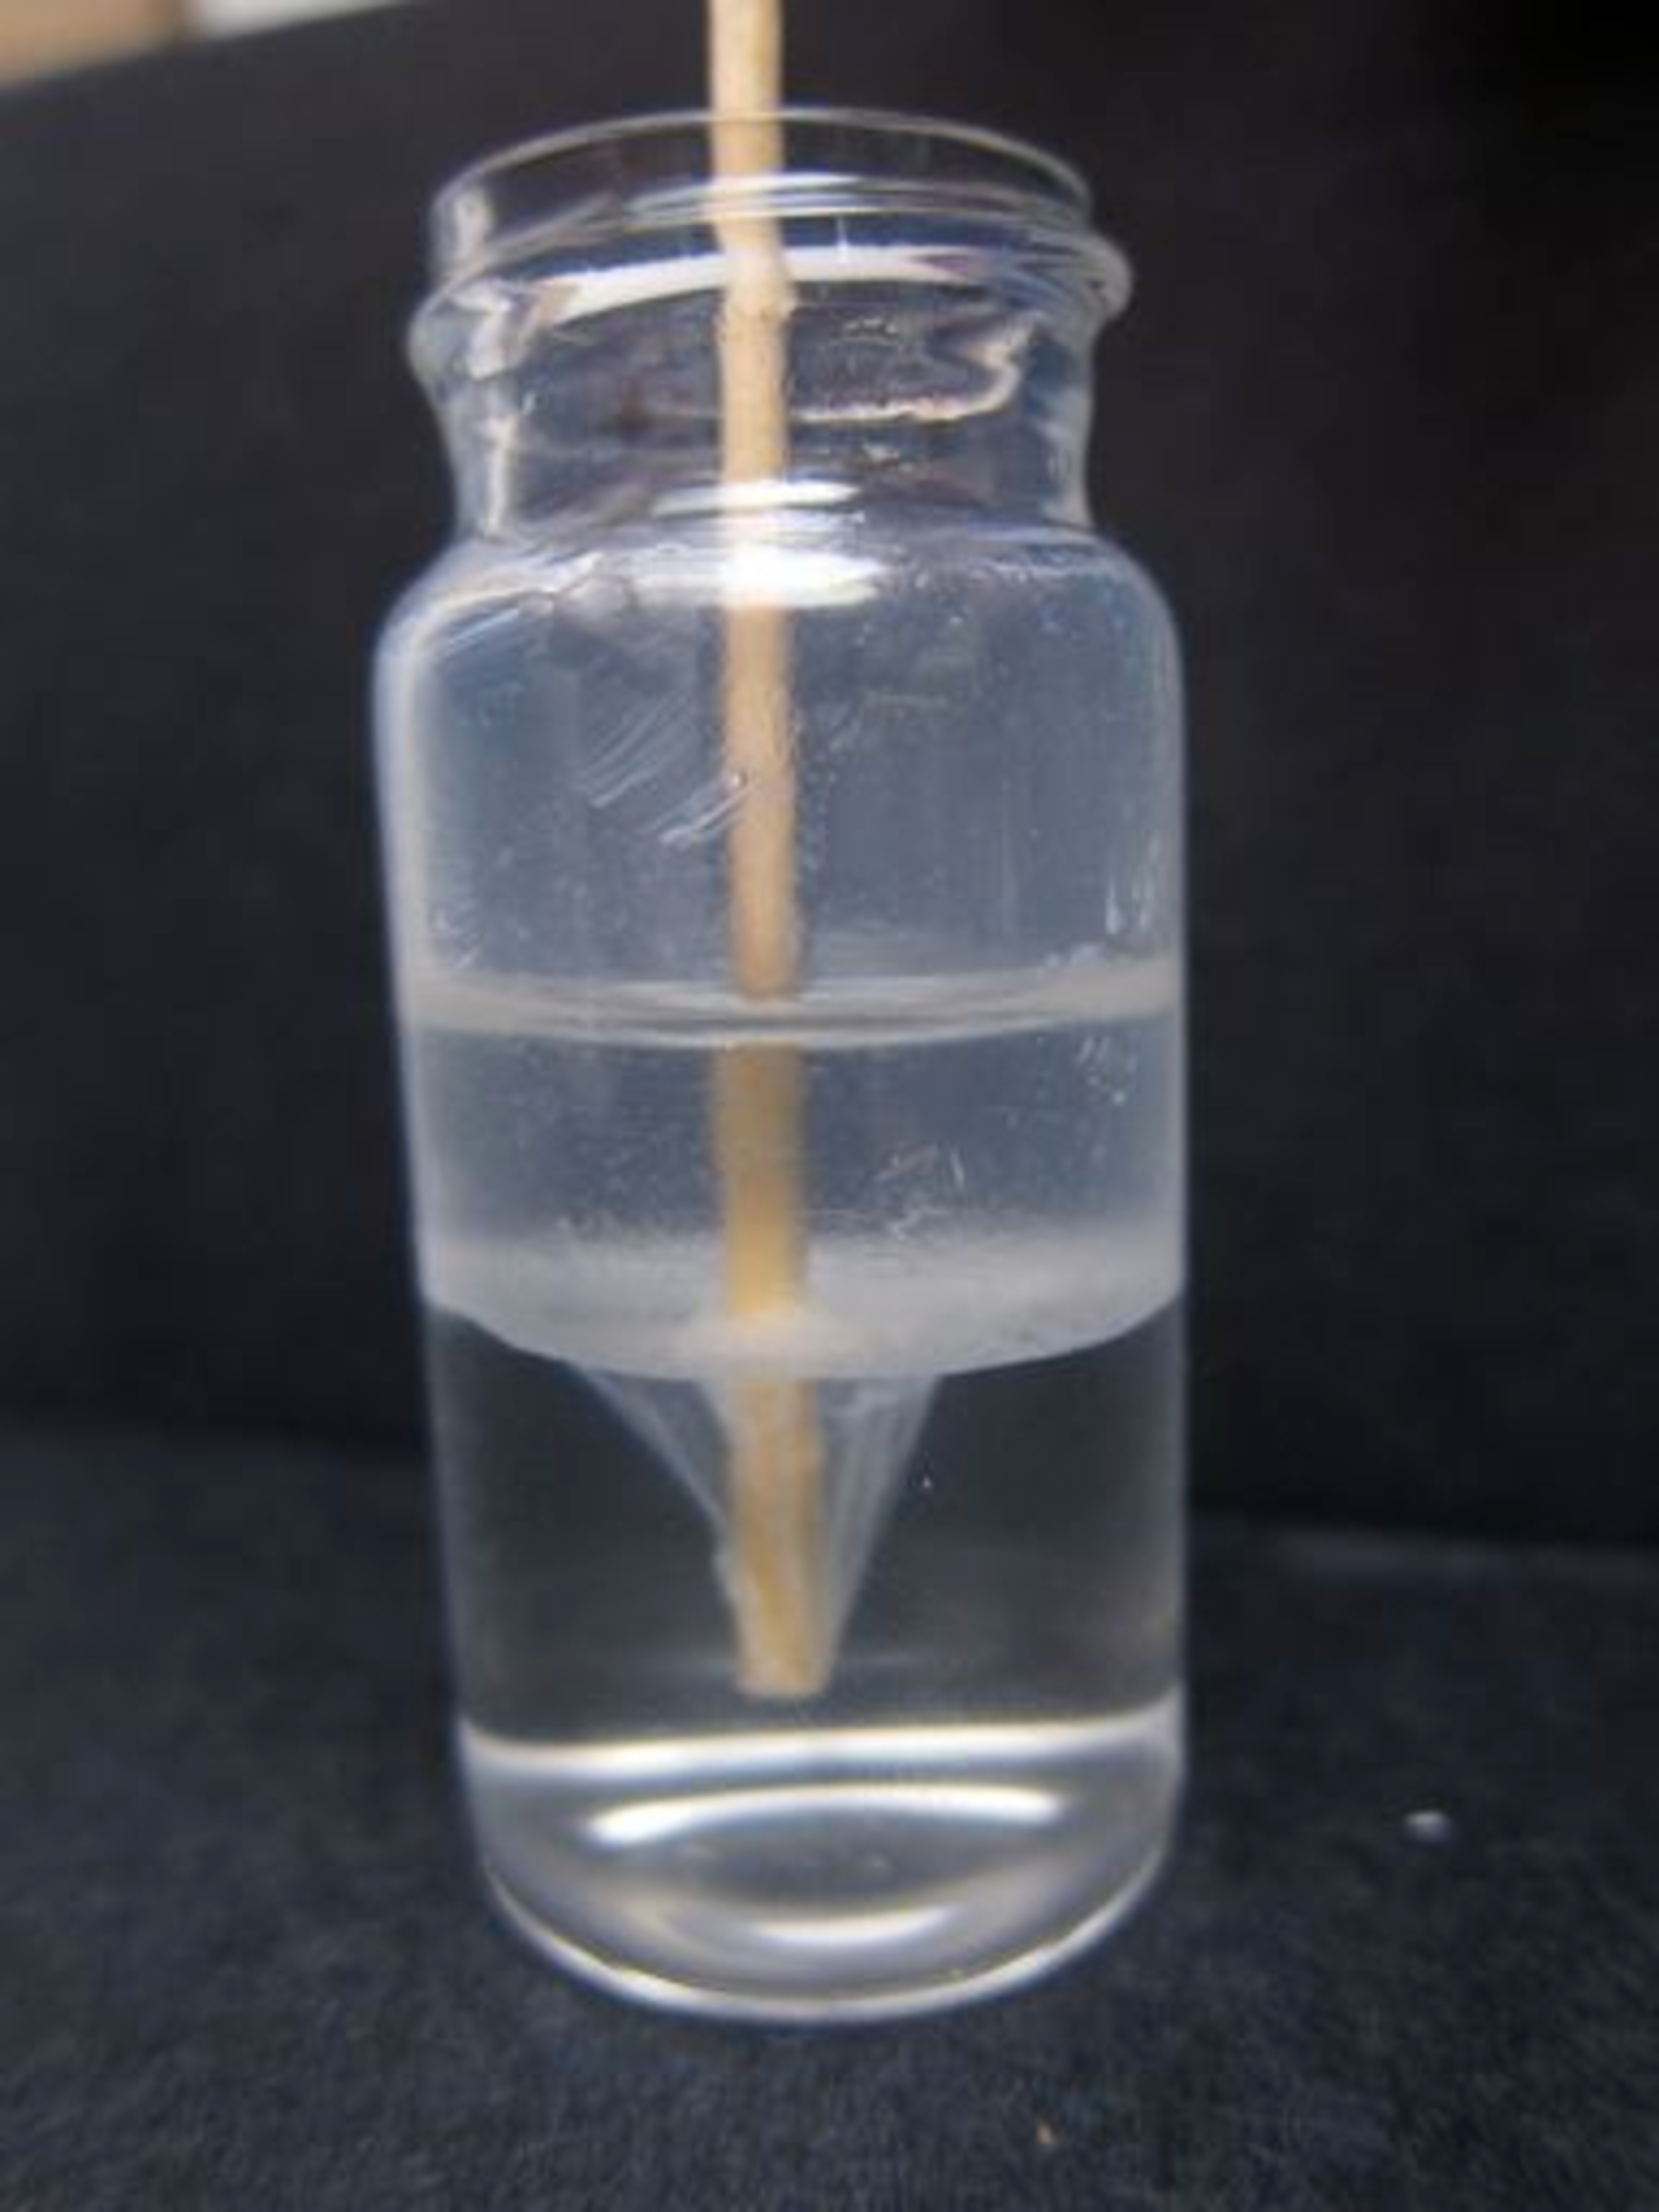
\includegraphics[width=1.25in]{figures/IMG_0912_reduced.pdf}
\hspace{0.2in}
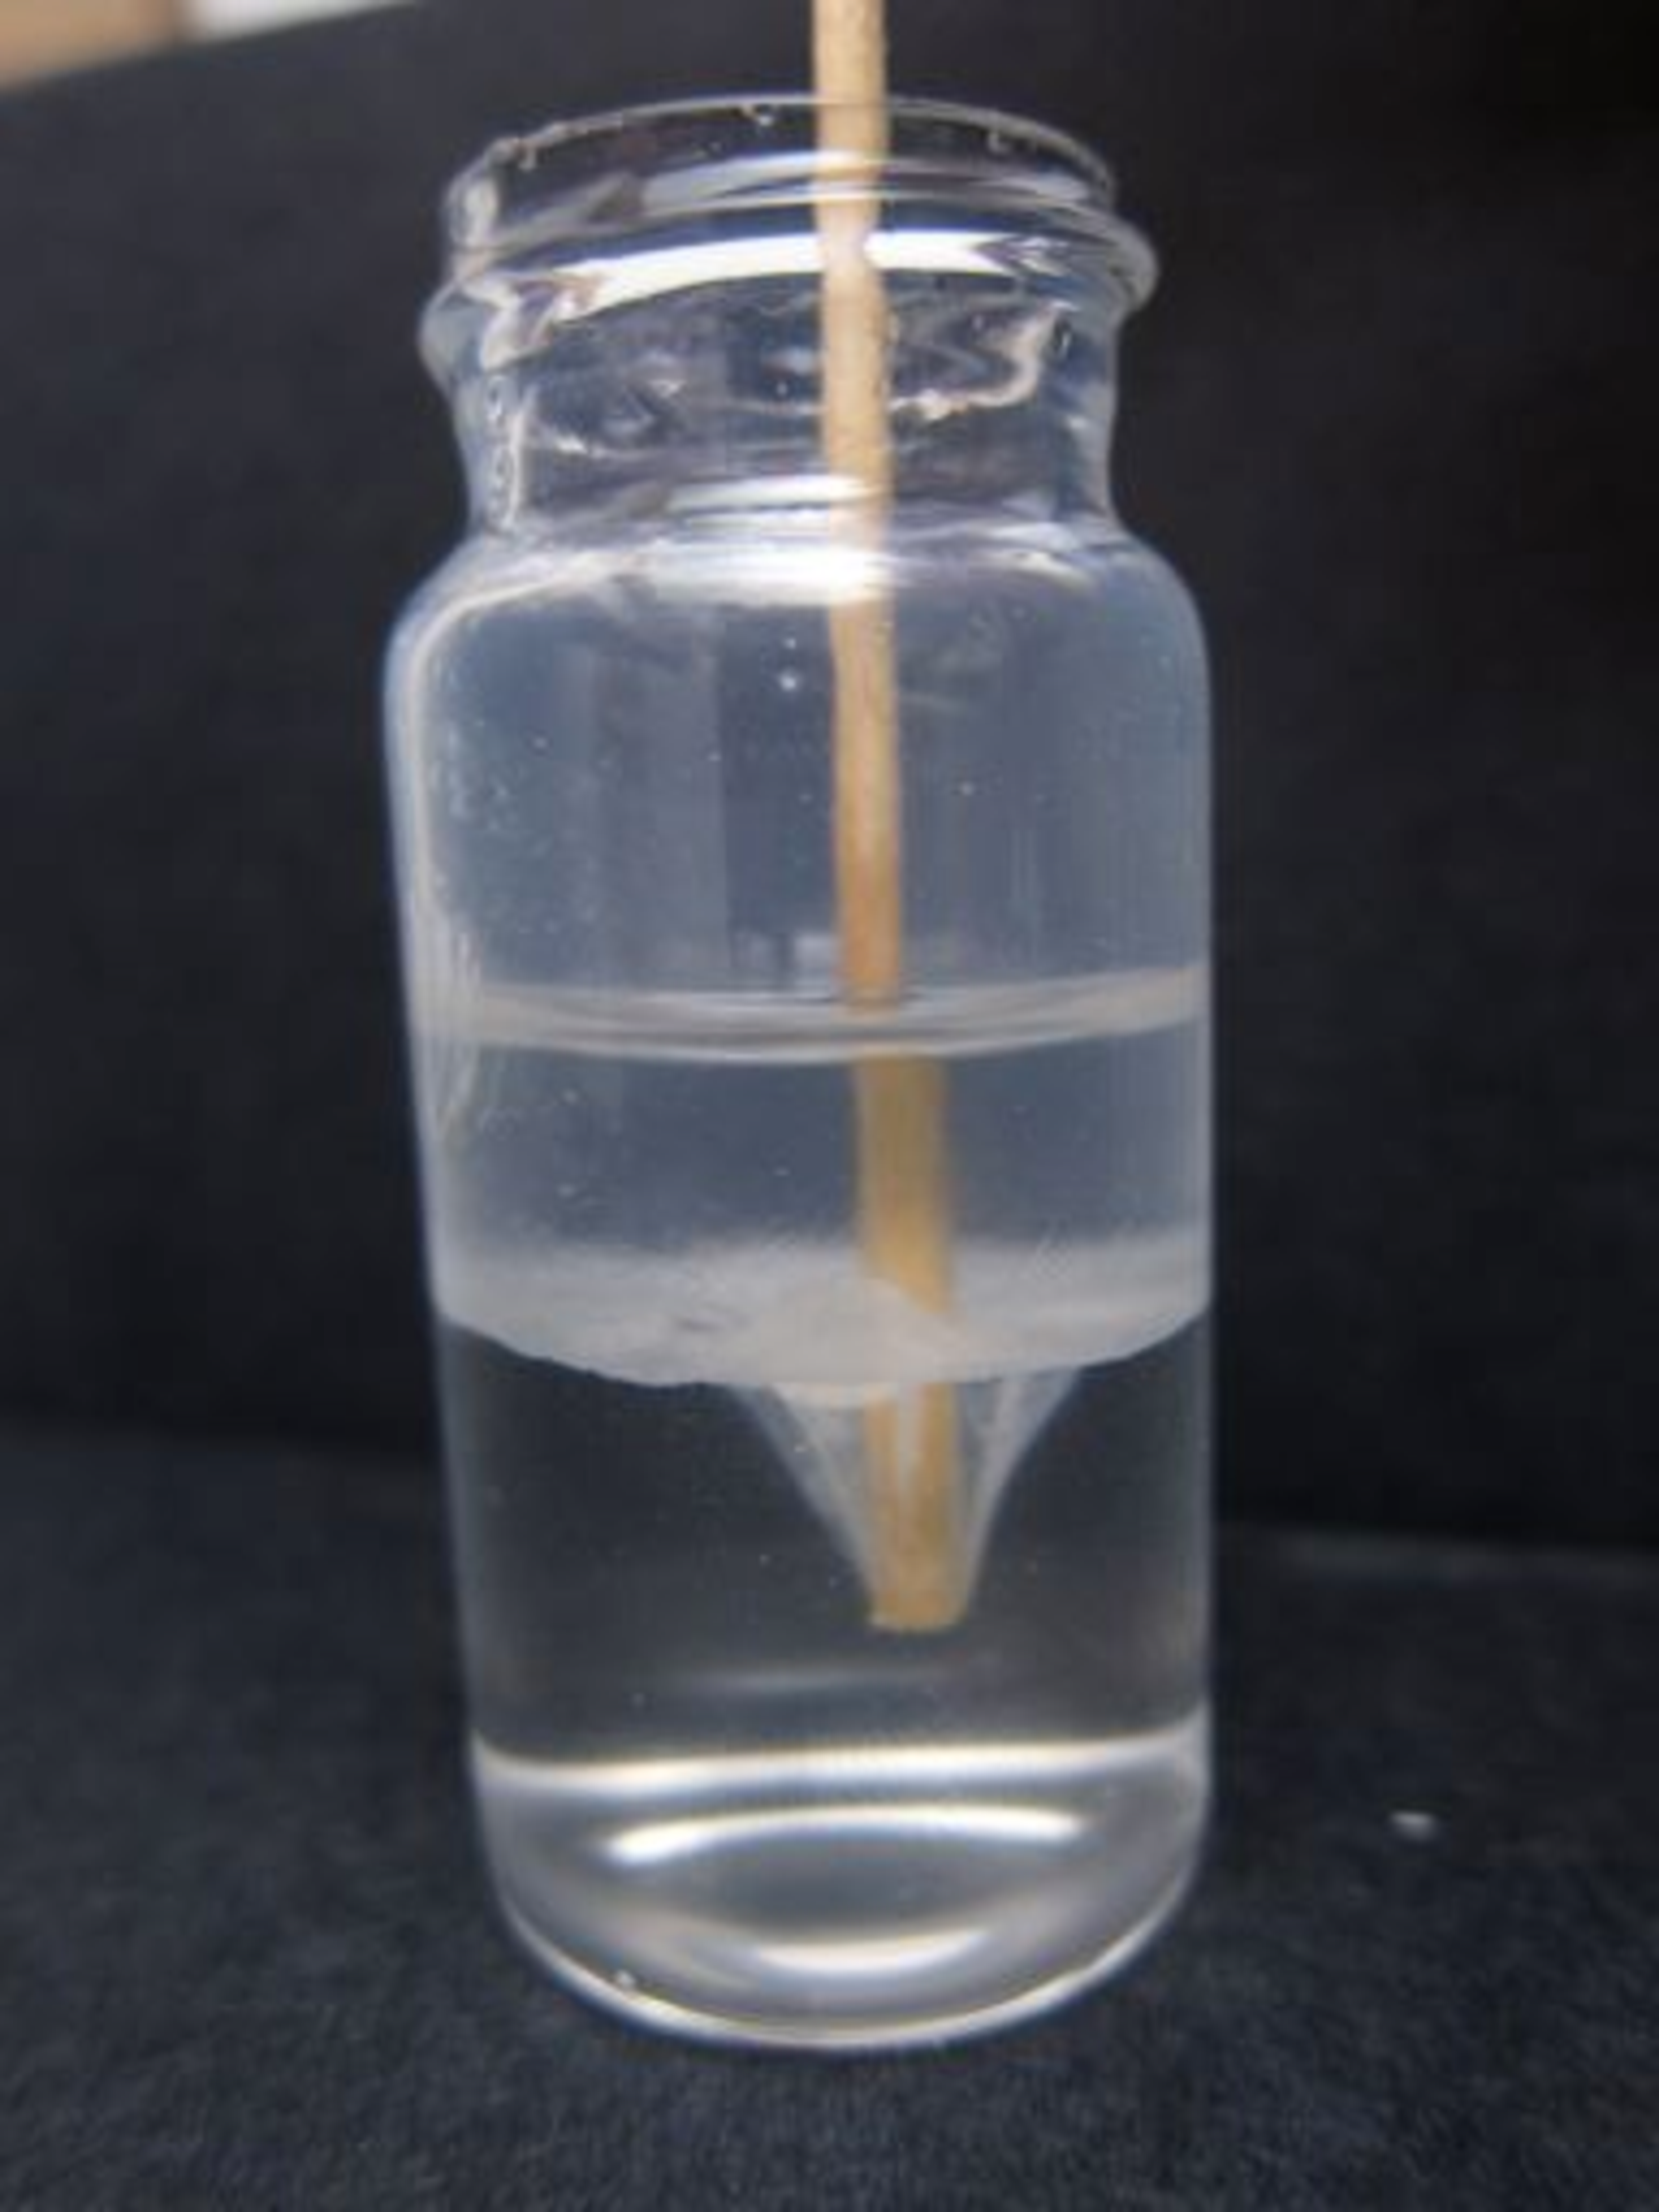
\includegraphics[width=1.25in]{figures/IMG_0913_reduced.pdf}
\hspace{0.2in}
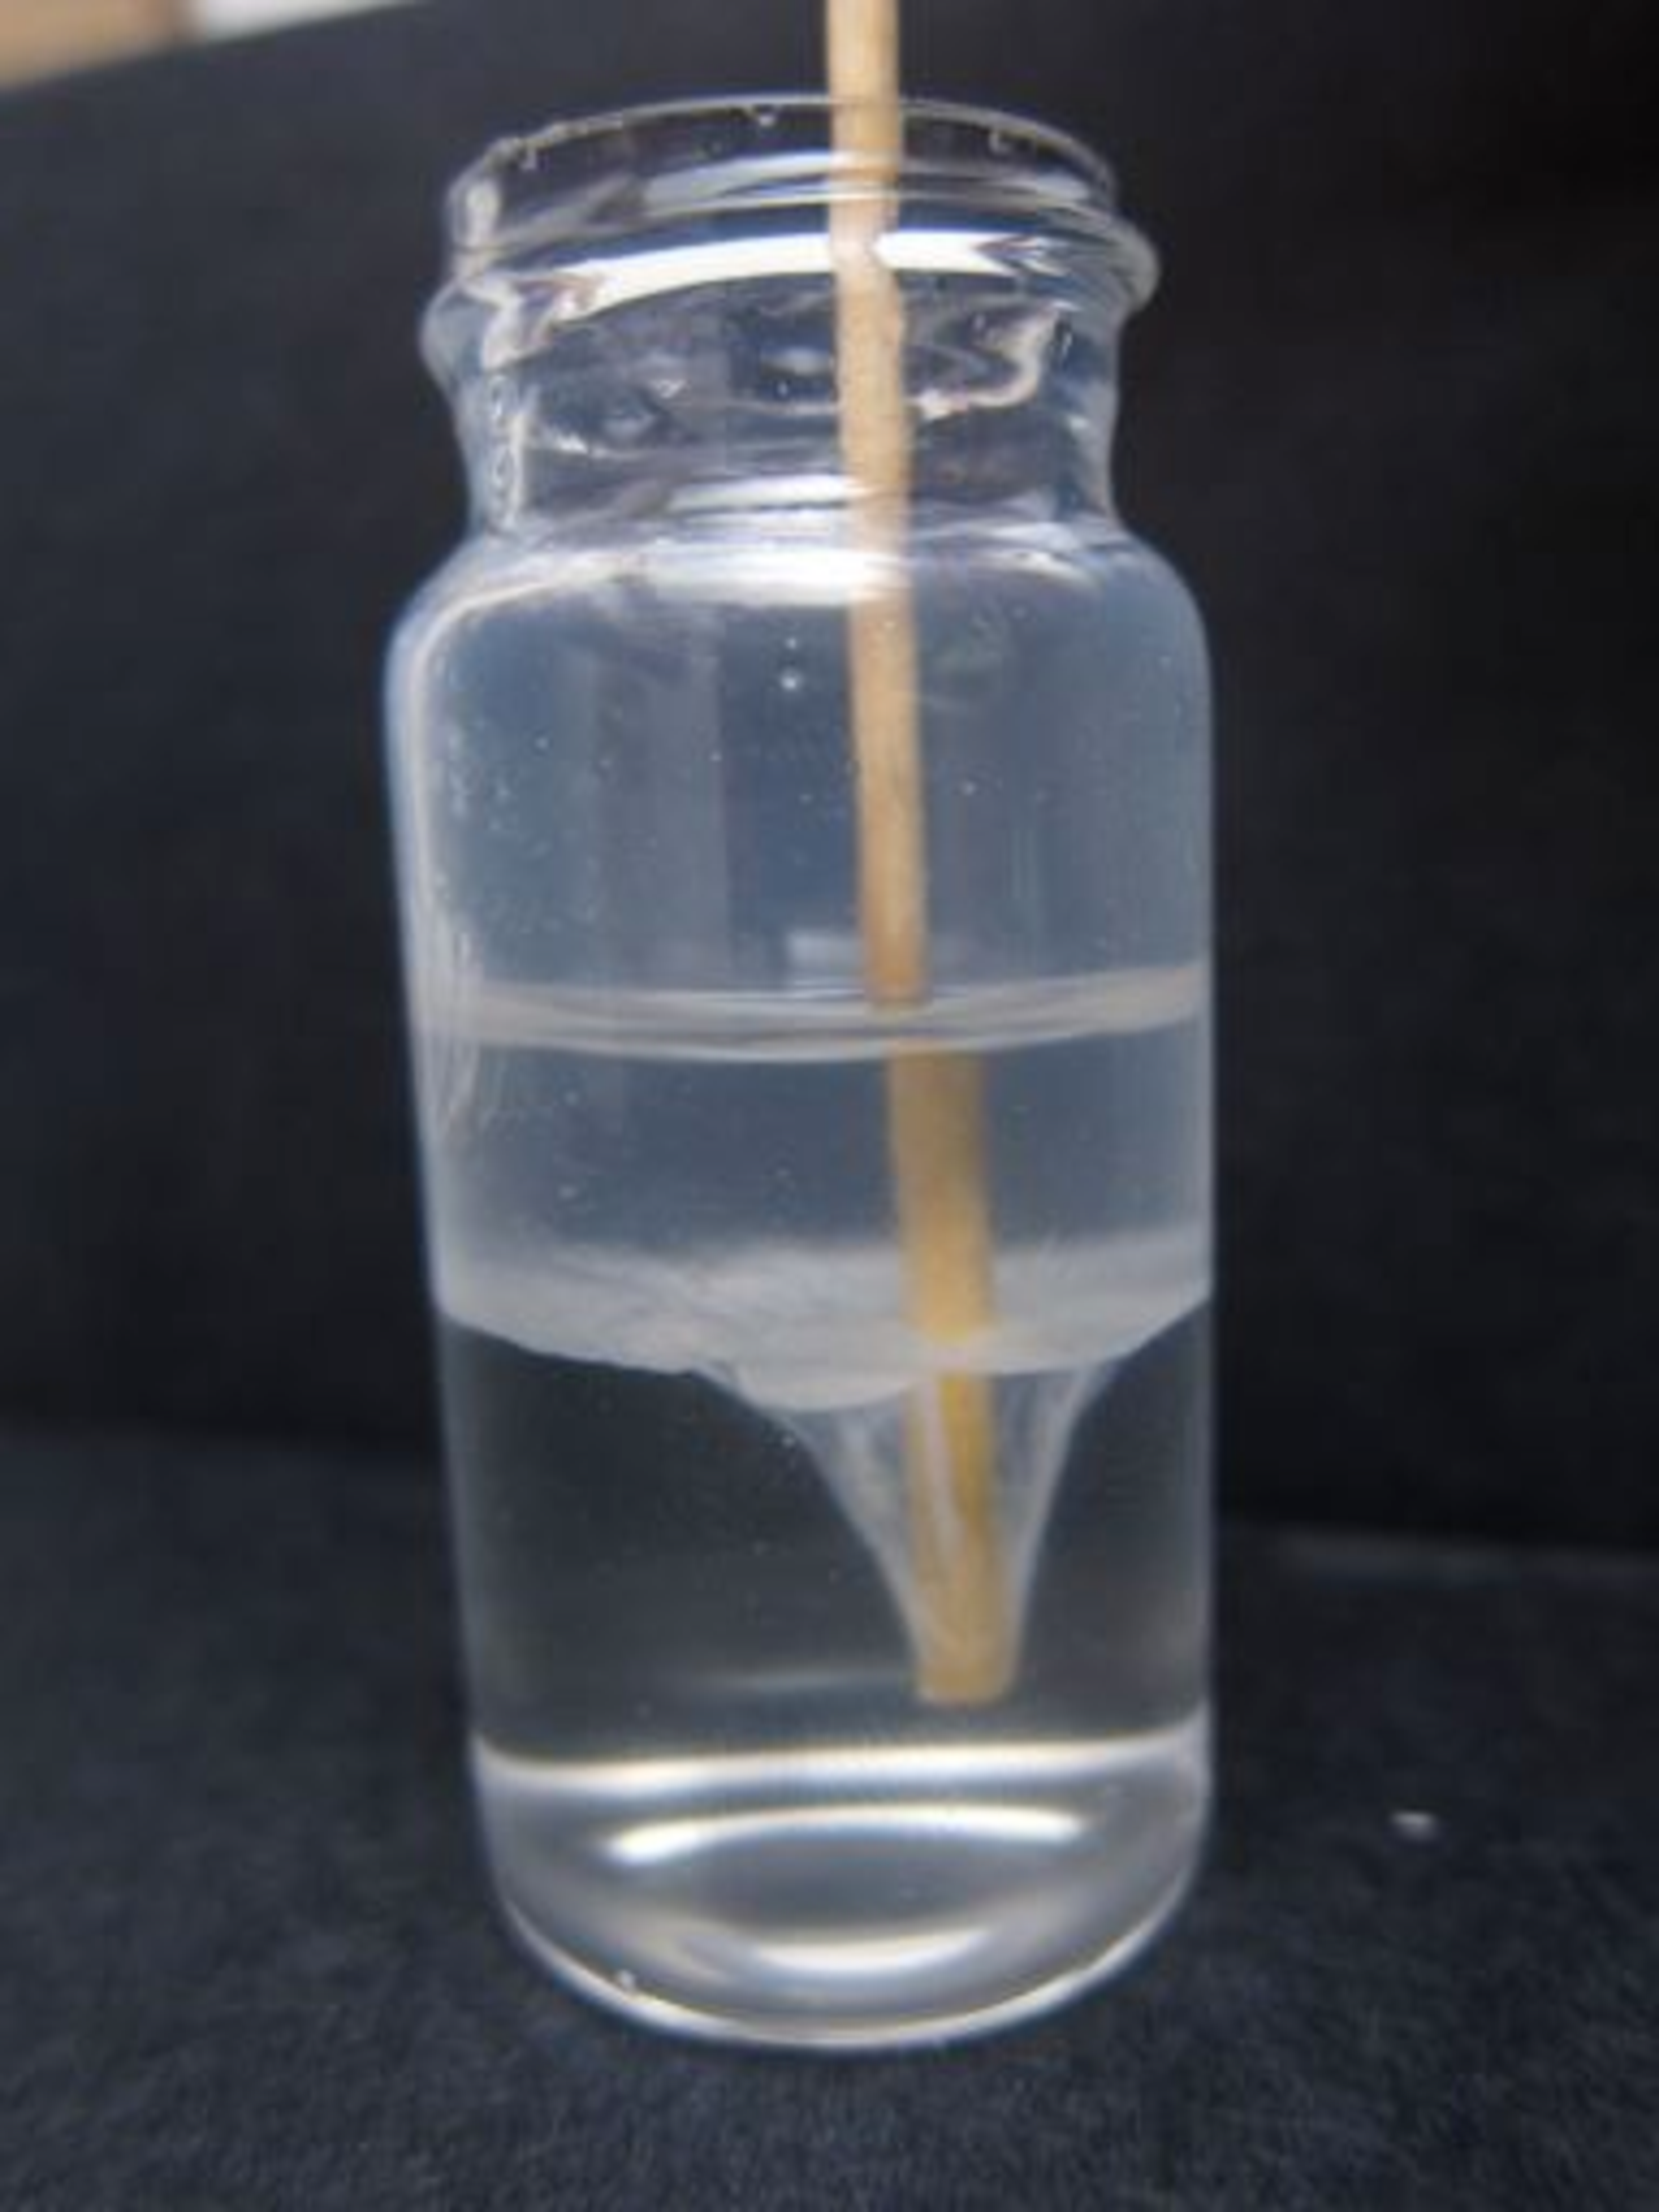
\includegraphics[width=1.25in]{figures/IMG_0914_reduced.pdf}
\caption{\label{fig:NDBinterface2} \emph{Amphiphilic dumbbells impart elasticity to an oil/water interface.}
Digital photographs of a membrane formed by amphiphilic dumbbells at a hexadecane/water interface being probed with a wooden stirrer.}
\end{figure*}

We have also observed amphiphilic dumbbells impart elasticity upon oil/water interfaces.
In Figure~\ref{fig:NDBinterface2} we see that the membrane formed by amphiphilic dumbbells at the interface between hexadecane and water is elastic enough to prevent a wooden stirrer from breaking through the interface.
As the stirrer is moved around, the dumbbell-covered interface deforms up to at least a centimeter while maintaining its integrity.
This procedure is reversible, the stirrer can be removed and reinserted many times without breaking through the interface.

The two demonstrations provided here suggest that amphiphilic dumbbells behave like colloidal surfactants and I expect that they will recapitulate many of the same phenomena.
Particularly, it would be interesting to explore the ability for dumbbells to stabilize emulsions.
Particle stabilized emulsions have been studied for more than a century (\cite{Ramsden:1903, Pickering:1907}) and are often referred to as Pickering emulsions.
So far, only spherical particles have been used to produce Pickering emulsions.
I suspect that the non-spherical shapes of dumbbells will result in emulsions with unique properties. Specifically, exploring the role of the size ratio of the two lobes in stabilizing droplets of different sizes would be very exciting.
Dumbbells with equally sized lobes should tend to stabilize larger droplets than dumbbells with one lobe significantly smaller than the other.


As we have seen, particles that are non-spherical can exhibit a variety of behaviors that spheres cannot.
Dumbbells, however, are just one type of anisotropic particle.
Another route to producing non-spherical particles that I have briefly explored is the compression of soft spheres to produce rhombic dodecahedra.
Adding a small amount of toluene, which is a good solvent for polystyrene and immiscible with water, to an aqueous suspension of polystyrene spheres causes the spheres to swell and soften.
Allowing the water to evaporate from this suspension generates a crystalline, usually face-centered cubic, packing of spheres which are eventually compressed by capillary forces as the final traces of water evaporate.
SEM images, like the one in Figure~\ref{fig:polygons}, of the final structure shows that after drying the compressed particles retain their polygonal shape.
The exact shape is presumed to be a rhombic dodecahedra since this is the space filling polygon that has the same unit cell as an FCC crystal of spheres.
If these polygons can be resuspended, it would be very interesting to study their self-assembly behavior, especially to see whether they will assemble into the densely-packed arrangement from which they were made or if they adopt some new structure accessible now due to their polygonal shape.
The structures formed by colloidal polyhedra are just beginning to be explored \cite{Henzie:2011}.


\begin{figure*}[htbp]
\centering
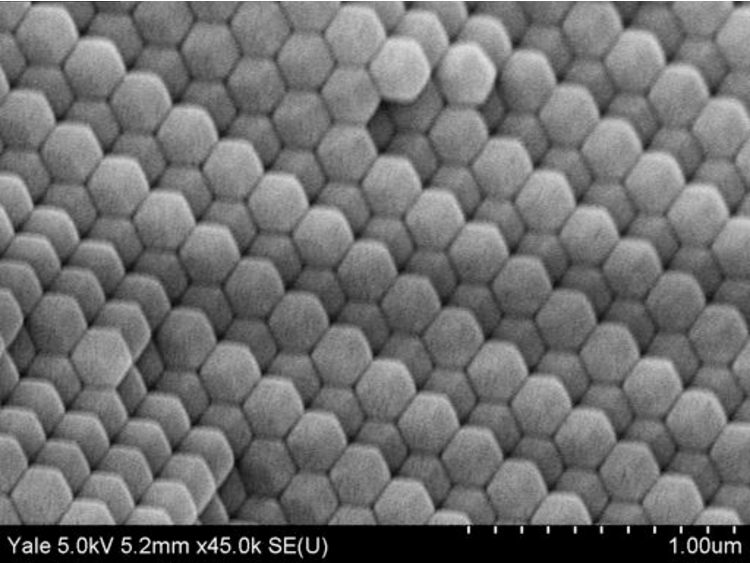
\includegraphics[width=.9\textwidth]{figures/B31_18_polygons.pdf}
\caption{\label{fig:polygons}\emph{Rhombic dodecahedra formed by capillary induced compression of toluene-swollen polystyrene spheres.}}
\end{figure*}












